\documentclass{article}

\usepackage{graphicx}

\title{Notes: An Effective Theory of $X^+-H$ Scattering}
\author{D. Odell}

\begin{document}

\maketitle

\section{Intro}

At low energies, the $X^+-H$ system can be considered a system of two particles
--- the $X^+$ particle does not ``resolve'' the $p-e$ structure of the $H$ atom.
However, as the $X^+$ particle approaches the $H$ atom, it induces a dipole,
which increases the attraction between the two ``particles''.
Induced dipole attraction goes like $-1/r^4$.
So, what happens when we model the $X^+-H$ system as a two-particle system that
interacts via an attractive $1/r^4$ potential?

Specifically,
\begin{itemize}
  \item If the bound-state spectrum of the $X^+-H$ system is a series of
low-energy states, shouldn't we be able to describe that spectrum with an
effective theory consisting of an attractive $1/r^4$ interaction and an
arbitrary short-range interaction?
  \item If I tune my system to reproduce the shallowest bound state, will I get the rest
of the spectrum?
  \item Are the $X^+-H$ bound states $1/r^4$ states? Specifically the ground
    state\ldots\ or is it associated with / affected by some other length scale?
\end{itemize}


\section{$\pi^+-H$}

\subsection{Local Regulator}

There are different ways we can choose to regulate the $1/r^4$ interaction and
define the short-distance pieces.
We will start with a purely local system where we can keep the number of states
fixed (is this cheating?).

Our interaction is
\begin{equation}
  \label{eq:local_interaction}
  V(r) = \left[1 - e^{-(r/R)^2}\right]^4 \left(-\frac{C_4}{r^4}\right) + g_{\rm
  LO} e^{-(r/R)^4}~,
\end{equation}
where we fix $C_4 = \lim_{r\rightarrow\infty} \alpha(r)/2 = 9/4$ and vary $g_{\rm LO}$ to reproduce the shallowest bound state for
each value of $R$.

Before we continue, it is worth discussing what we're comparing to.
Lazuaskas and Carbonell already did a two-body calculation (before surpassing
it with a proper three-body calculation) using the Mott-Massey potential
\begin{equation}
  \label{eq:mott_massey}
  V_{\rm MM}(r) = -\frac{\alpha(r)}{2r^4}~,
\end{equation}
where 
\begin{equation}
  \label{eq:alpha}
  \alpha(r) = \frac{9}{2} - \frac{2}{3} e^{-2r}\left( r^5 + \frac{9}{2}r^4 +
  9r^3 + \frac{27}{2}r^2 + \frac{27}{2}r + \frac{27}{4} \right)~.
\end{equation}

The shallowest bound state (sixth excited state) lies at $B_2^{(6)}=1.20\times~10^{-4}$~a.u.
This is the state we will tune with $g_{\rm LO}$.
Then we will compare the rest of the spectrum to the spectrum found with $V_{\rm
MM}$.

The Renormalization Group (RG) flow is shown Figure~\ref{fig:rg_flow}.
This is, of course, just one of an infinite number of branches, each with a unique
number of bound states. 
There are 7 states in this branch.

\begin{figure}
  \centering
  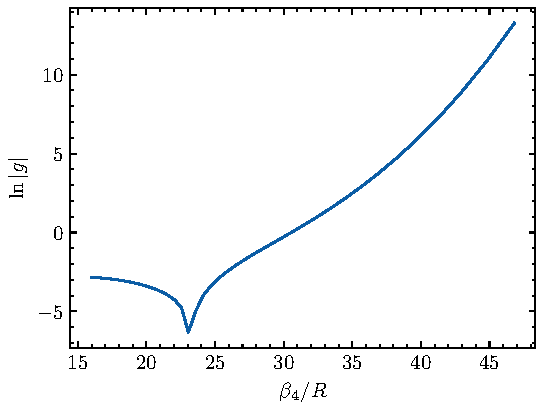
\includegraphics{figures/rg_flow.pdf}
  \caption{The running of the counterterm strength, $g$, as the short-distance
  cutoff, $R$, goes to zero. $B_2^{(6)}$ was kept fixed as $R$ was varied. $g$
is negative to the left of the ``dip''. $\beta_4\equiv~(2\mu
C_4)^{1/2}$.}\label{fig:rg_flow}
\end{figure}

Only $B_2^{(6)}$ is fixed in this calculation.
The other binding energies have significant $R$ dependence.
The hypothesis here is that they will stabilize near the $V_{\rm MM}$ results.
From Figure~\ref{fig:B2s}, two things are expected:
\begin{itemize}
  \item Disagreement grows with energy. The further away the state is from the
    sixth excited state, the worse the agreeement. This is expected from an
    effective theory.
  \item The asymptotic values of $B_2^{(n)}$ for $n<4$ are very far from the $V_{\rm
    MM}$ results.
\end{itemize}

\begin{figure}
  \centering
  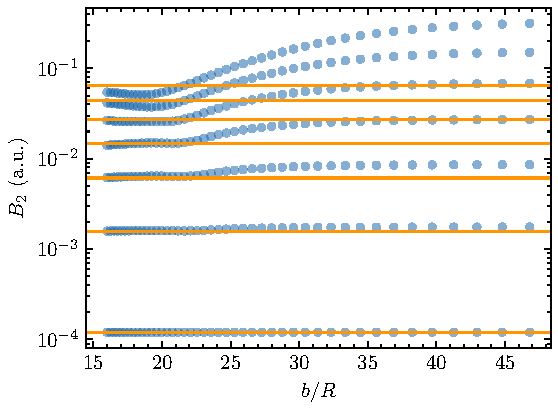
\includegraphics{figures/B2s.pdf}
  \caption{Binding energies as $R$ goes to zero. Blue circles represent the
    effective theory calculation. Orange lines represent the spectrum found with
  $V_{\rm MM}$. The shallowest state's agreement is by design.}\label{fig:B2s}
\end{figure}


In light of the second point, it is worth looking at the energy dependence of
the deviations, shown in Figure~\ref{fig:B2_rel_diffs}.
Here we see a nearly linear dependence on $B_{2,{\rm MM}}$.
The ground state seem to deviate from the linear trend.

\begin{figure}
  \centering
  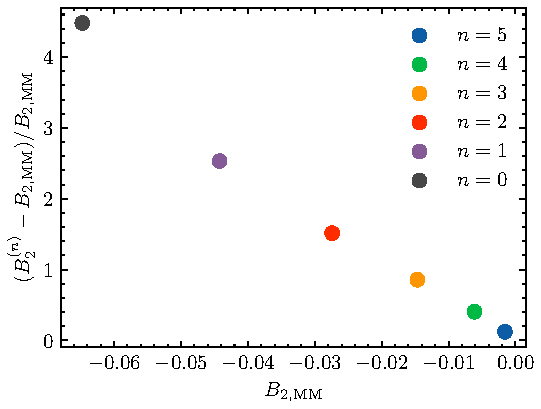
\includegraphics{figures/B2_rel_diffs.pdf}
  \caption{Relative differences of the binding energies as the states get
  deepeer. The zero crossing for $n=6$ (blue circle) is again by
design.}\label{fig:B2_rel_diffs}
\end{figure}

It is important to note that the values shown in Figure~\ref{fig:B2_rel_diffs} are
extrapolated.
The convergence of each state (other than the sixth excited state) is shown in
Figure~\ref{fig:B2_convergence_panels}.
A simple fit was done to extract an asymptotic value where the curves are
assumed to follow the form
\begin{equation}
  E_2(R) = C_1 + C_2 e^{-C_3 R}~,
\end{equation}
where $C_m$ are fit.
$C_1$ values are shown in~Figure~\ref{fig:B2_convergence_panels}.

\begin{figure}
  \centering
  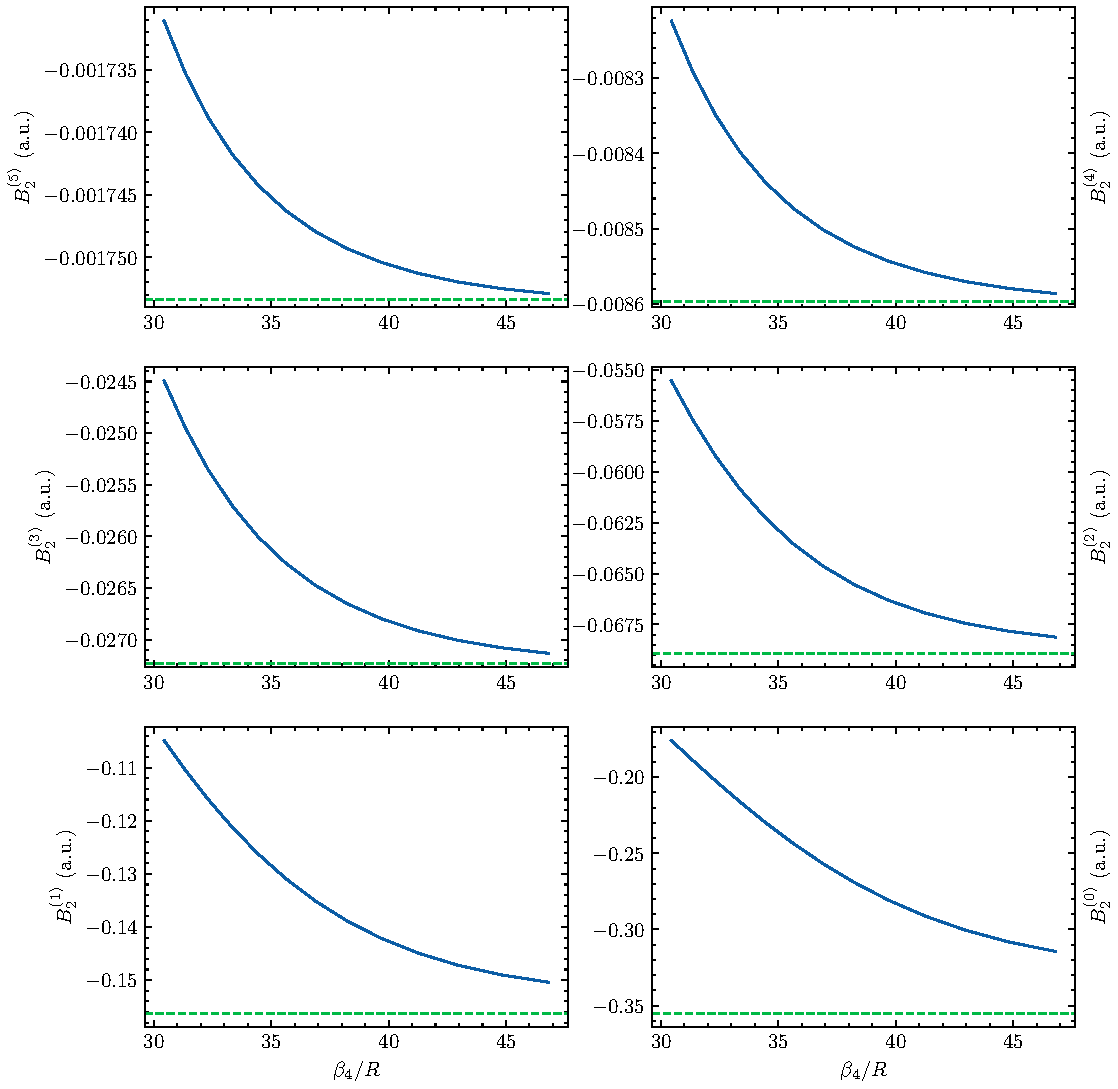
\includegraphics[width=\linewidth]{figures/B2_convergence_panels.pdf}
  \caption{Convergence of deeper states as $R$ goes to zero. Blue lines
  represent the effective theory calculation. Green lines represent the
extracted asymptotic values.}\label{fig:B2_convergence_panels}
\end{figure}

\subsection{Why Doesn't This Work Better?}

The electron binding energy is approximately 0.5 a.u.
If that is the relevant breakdown scale (?), then the states we are trying to
predict with our effective theory are easily considered ``low-energy''.
We ought to be doing better than this at leading order (LO).

Below, in Figures~\ref{fig:V_comparison} and~\ref{fig:V_rel_comparison},
the effectiver potential (without a counterterm) is shown in comparison to the
Mott-Massey potential.
Figure~\ref{fig:V_comparison} shows the absolute comparison while
Figure~\ref{fig:V_rel_comparison}.
For Figure~\ref{fig:V_comparison}, $R = 1.5$ a.u.
This is approximately where the predictions match the MM spectrum as seen in
Figure~\ref{fig:B2s}.
For Figure~\ref{fig:V_rel_comparison}, a range of $R$ values is shown.
Beyond $r\approx~5$~a.u., is seems that the potentials are nearly identical.
(Perhaps this tells us something about the breakdown scale?)

\begin{figure}
  \centering
  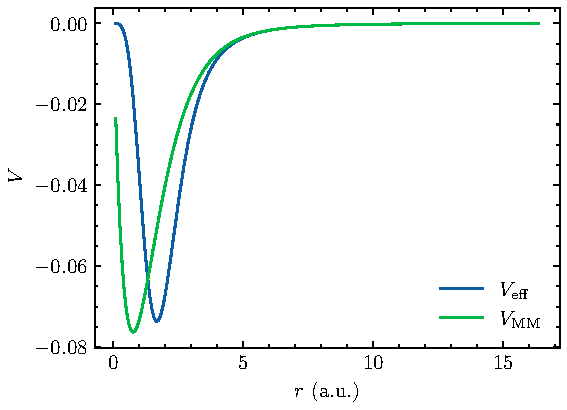
\includegraphics[width=\linewidth]{figures/V_comparison.pdf}
  \caption{Comparison of the regulated $1/r^4$ and Mott-Massey
potentials at $R=1.5$.}\label{fig:V_comparison}
\end{figure}

\begin{figure}
  \centering
  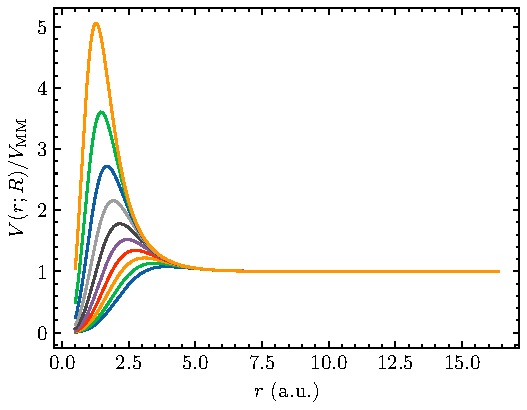
\includegraphics[width=\linewidth]{figures/V_rel_comparison.pdf}
\caption{Relative comparison of the regulated $1/r^4$ and Mott-Massey
potentials for a range of $R$ values.}\label{fig:V_rel_comparison}

\end{figure}

\end{document}
